\documentclass[12pt]{article}
\usepackage[left=0.5in, right=0.5in, top=0.5in, bottom=0.5in]{geometry}
\usepackage{algpseudocode}
\usepackage{algorithm}
\usepackage{graphicx}
\graphicspath{ {./} }

\title{\textsc{CS180 Midterm}}
\author{Henry Trinh}

\begin{document}
\maketitle 
\begin{center}
    \textbf{UID:} 105101098
    
    Discussion 1B
\end{center}

\newpage
\section*{Problem 1}
\subsection*{Part A}
\textbf{True}, if an edge $e$ disconnects a connected graph $G$, a DFS on $G$ will always
a tree in such a way that $e$ will be a tree edge since the edge will be guaranteed
to be visited to visit every node. A tree edge is an edge that is present in the tree 
resulting from a DFS on a graph, and thus, edge $e$ will be a tree edge.
\subsection*{Part B}
\textbf{False}, this is not necessarily true. Only the node with no incoming edge will have
its place defined in a topological ordering. For a counter example, we have a DAG $G$ with three
nodes: $A$, $B$, $C$. In our example, $G$ has two directed edges, $(A, B)$ and $(A,C)$, such that
node $A$ is the only node with no incoming edge. Two valid topological orderings are 
$A-B-C$ and $A-C-B$.
\subsection*{Part C}
\textbf{False}, this is not alwasy the case. We can prove that this statement is False
by providing an example. Given an example with two males and two females with preferences 
${m_1: w_2 > w_1}$, ${m_2: w_2 > w_1}$, ${w_2: m_2 > m_1}$, ${w_1: m_2 > m_1}$, if we 
perform stable matching, $(m_1, w_2)$ will be in a stable matching.
\subsection*{Part D}
\textbf{True}. Given a DAG $G$ and we know that the nature of doing a DFS is that it checks one branch
at a time. If node $u$ is the first leaf node visited, it will not have any outgoing edges 
because if there is an outgoing edge to an unvisited node, then node $u$ is not a leaf node. If 
there is an outgoing edge to a visited node, then this contradicts the fact that $G$ is acyclic
because $G$ would then have a cycle.

\newpage
\section*{Problem 2}
$f_5(n)$, $f_2(n)$, $f_1(n)$, $f_4(n)$, $f_3(n)$
\newline
\begin{center}
    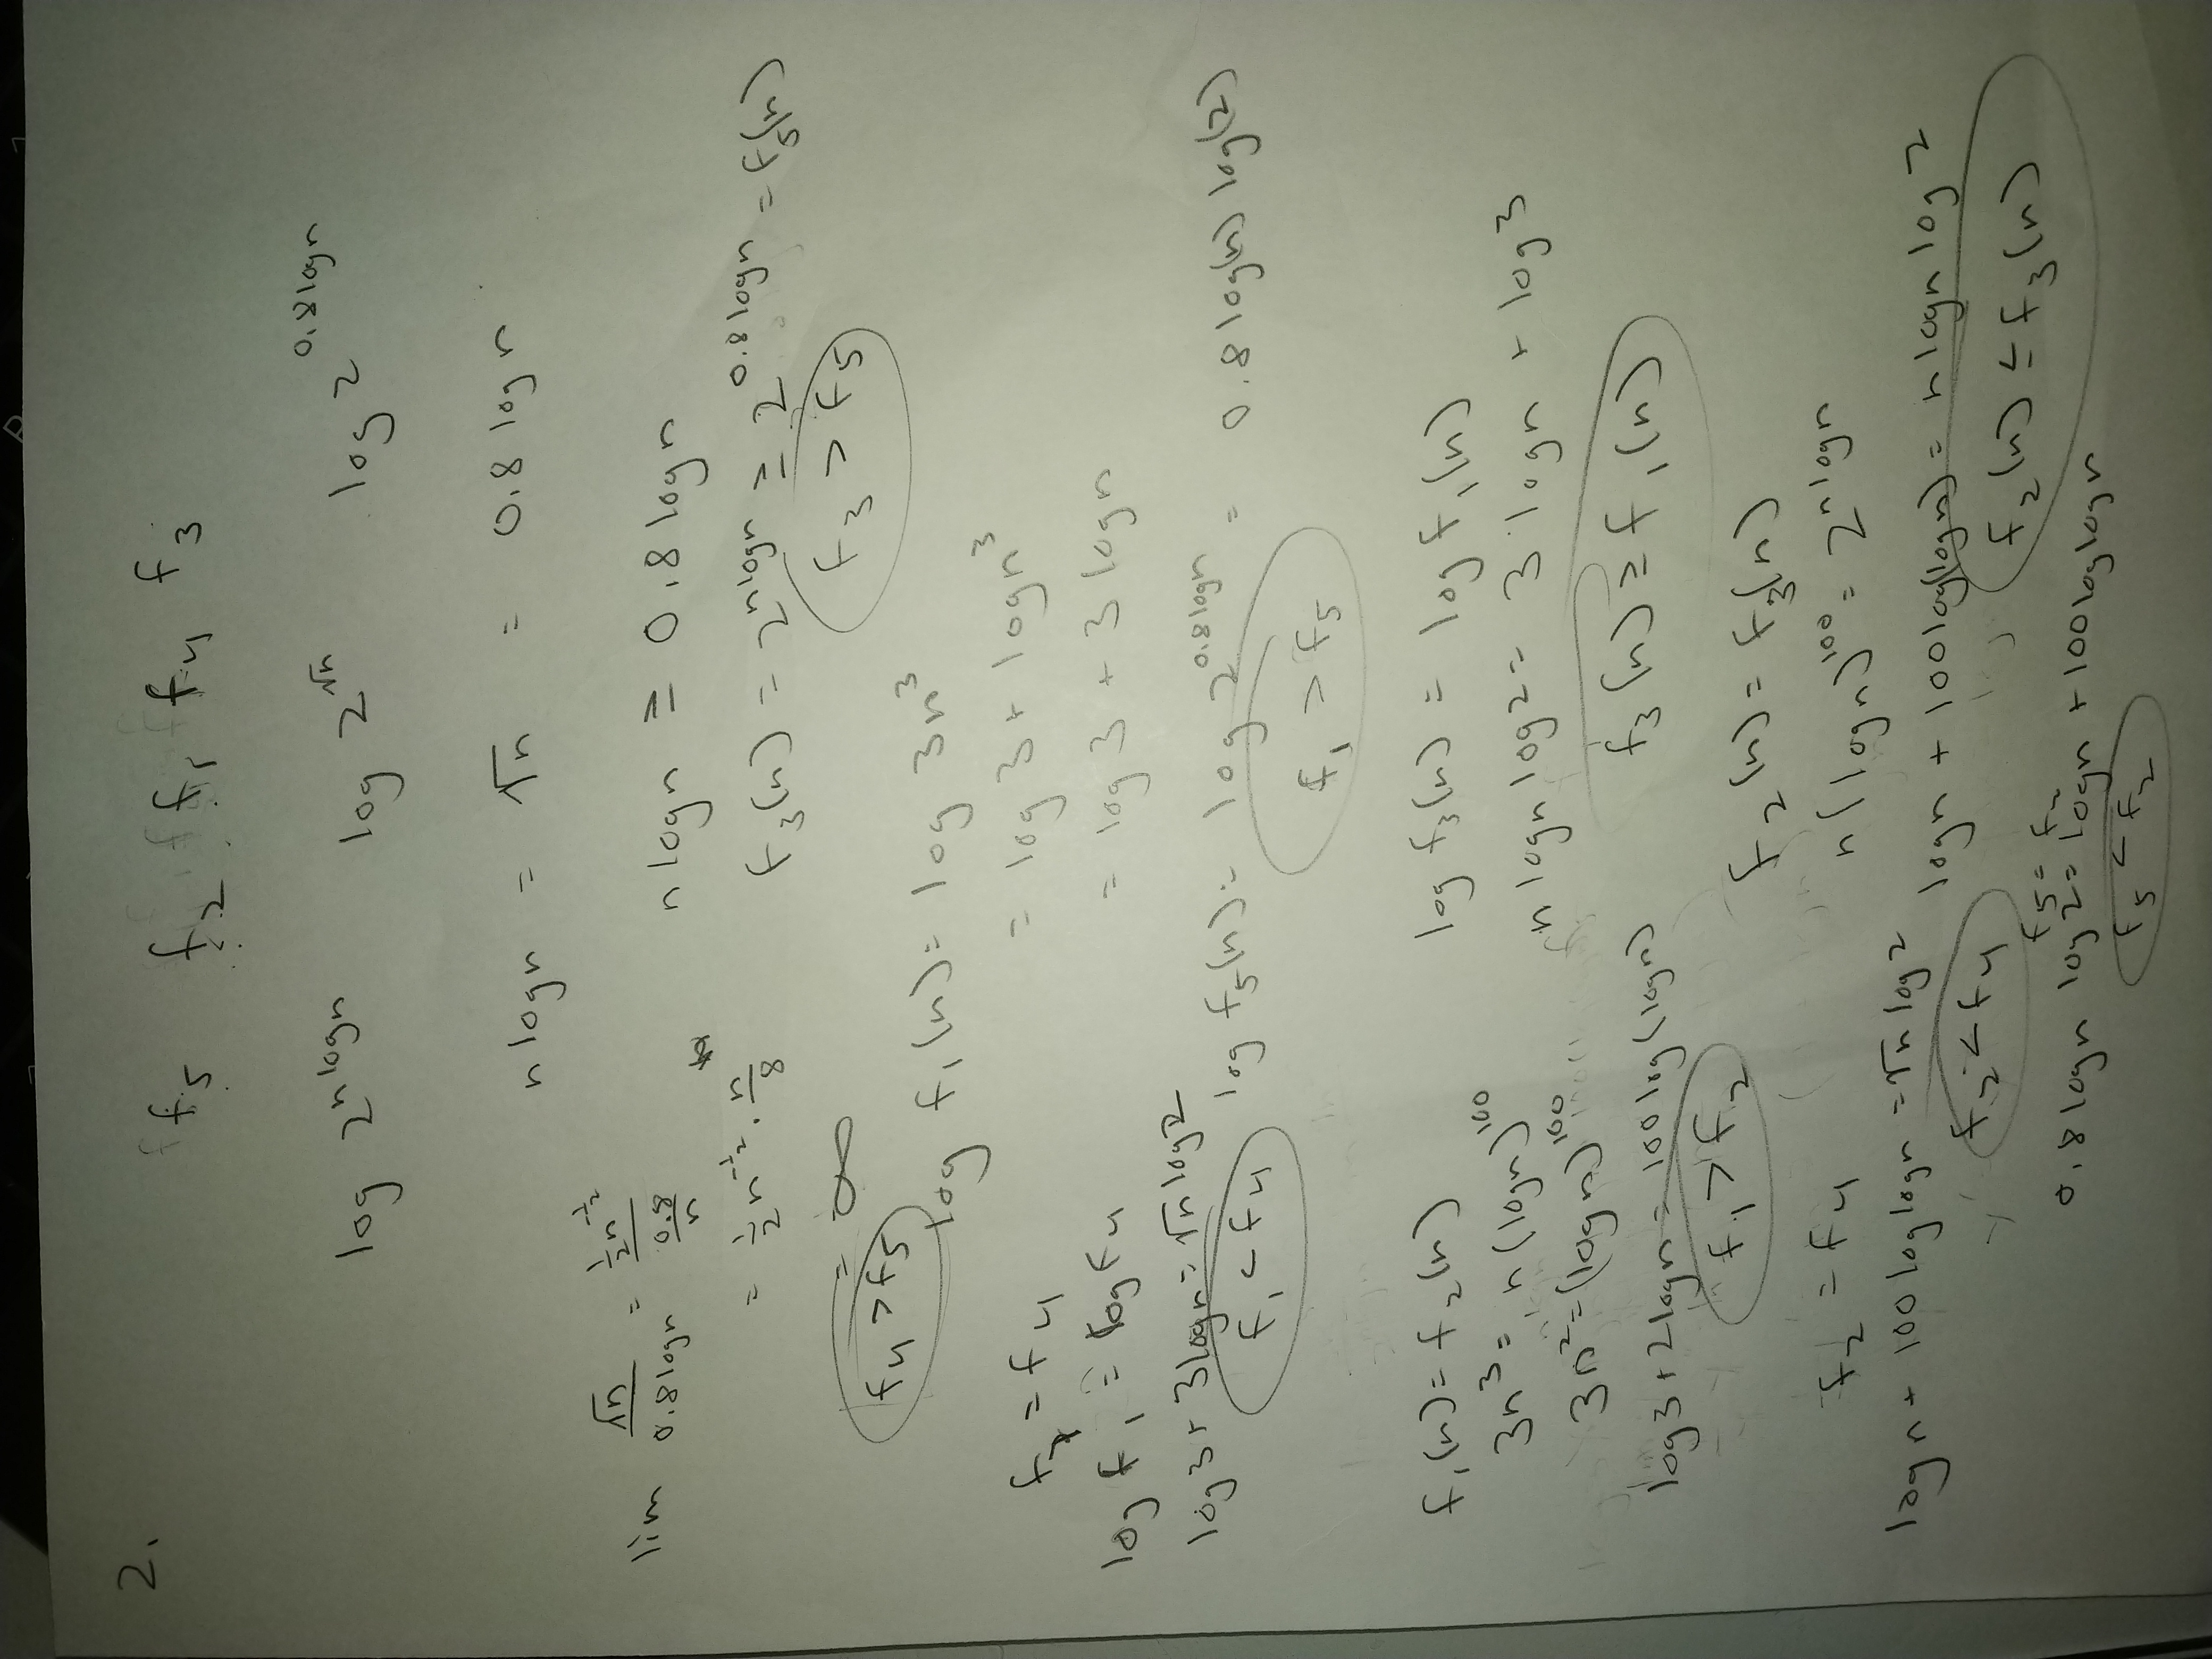
\includegraphics[scale=0.155, angle=270]{hi.jpg}
\end{center}


\newpage
\section*{Problem 3}
\begin{algorithm}
\caption{Test if there exists a path in DAG that visits each node once.}
\begin{algorithmic}[1]
\State $topArr \gets $ array of nodes returned from topological sort on DAG $G$
\For {$i$ in $topArr$}
    \If {$(topArr[i], topArr[i+1]) \notin E$}
        \State return false
    \EndIf
\EndFor
\State return true
\end{algorithmic}
\end{algorithm}
Since graph $G$ is a directed acyclic graph, there exists a topological sort. For there to be a path that
visits each node exactly once, we must find if there exists a hamiltonian path. This can only be true
if there exists an edge bewteen a node $i$ and $i+1$ in the topological sort of $G$ for any $i$. If there
is a pair of nodes $i$ and $i+1$ for any given $i$ there would be no path that connects all nodes since
the only nodes that can be directed towards $i+1$ are the nodes before it in a topological sort.

\newpage
\section*{Problem 4}
\begin{algorithm}
\caption{Find if there is index $i$ such that $A[i]=i$}
\begin{algorithmic}[1]
\State $left \gets 0$ 
\State $right \gets length(A) - 1$
\While {$left < right$}
    \State $middle \gets ((right-left)/2) + left$
    \If {$A[middle] = middle$}
        \State return true
    \EndIf
    \If {$A[middle] < middle$}
        \State $left \gets middle + 1$
    \Else 
        \If {$A[middle] > middle$}
            \State $right \gets middle - 1$
        \EndIf
    \EndIf
\EndWhile
\State return false
\end{algorithmic}
\end{algorithm}
This algorithm employs a binary search in an array $A$ in order to find if there is an index $i$ such
that $A[i]=i$. By utilizing a binary search instead of a linear traversal, we can search in $O(logn)$ 
instead of $O(n)$. If the current proposed index $i$ is less than $A[i]$, we continue the binary search
with the lower half of the array because it is impossible to find $i$ where $A[i]=i$ in the latter half
even if $A[i]$ increases by only $1$ per index. Vice versa, we do the opposite if $A[i]<i$.

\newpage
\section*{Problem 5}
\begin{algorithm}
\caption{minimum number of lasers to destroy all saucers}
\begin{algorithmic}
\State $A \gets $ array of intervals given by sorting all intervals by $R_i$ in increasing order
\State $S \gets $ empty Set
\State $X \gets $ empty Set
\ForAll {$(L, R)$ in $A$}
    \If $(L, R) \in S$
        \State continue with loop
    \EndIf
    \State put $R - 0.5$ in $X$
    \State put all $(L, R)$ that contains $R - 0.5$ in $S$
\EndFor
\State return $X$
\end{algorithmic}
\end{algorithm}
This problem can be solved using a greedy algorithm approach. If we are able to sort the intervals
by increasing order of the value at which each interval ends, which is an O(nlogn) operation, we are 
able to utilize the $R$ of an interval not visited yet with the smallest valued $R$ as a "laser" point, $x_n$. This works
because with utilizing the current lowest R would be an optimal local solution for trying to hit as many
saucers(intervals) as possible with one laser. By doing this, we can optimize the amount of intervals hit
per laser point proposed. This algorithm would take $O(nlogn)$ time because of sorting. Marking the set $X$,
the set of laser points, is only a linear traversal.

\end{document}